% 第2章
%!TEX root = main.tex
本章では,実験を行なった開発機体の開発コンセプトと,設計や搭載システムの概要を述べる.機体は,災害発生時,回転翼機モードで離陸し,上空で固定翼機モードへと遷移して被災地へ向かう.そして被災地上空へ到着した後,回転翼機モードへと遷移し,ホバリング飛行しながら,情報収集や着陸可能地点の検出を行なう.

\section{実験機の概要}
本研究グループの目的である,大規模災害発生時の任務遂行には,狭隘地への進入が必要な場合がある.また救援物資の運搬に利用する場合,救助者に近い距離で着陸を行なう可能性もあり,対人安全性の強化が必要である.さらに,空撮や着陸可能地点の検出には,安定した飛行とホバリングを行なう必要がある.

以上を踏まえて,機体製作にあたり以下の3点
	\begin{enumerate}
	\item 機体サイズの小型化
	\item 対人安全性を考慮
	\item ヘリコプタと同等のホバリング性能
	\end{enumerate}
をコンセプトとしている.2015年に,エアロセンス株式会社と共同開発を行なったが,本研究ではFig. \ref{fig:vtol23k}に示す後継機を用いている.

\begin{figure}[H]
\centering
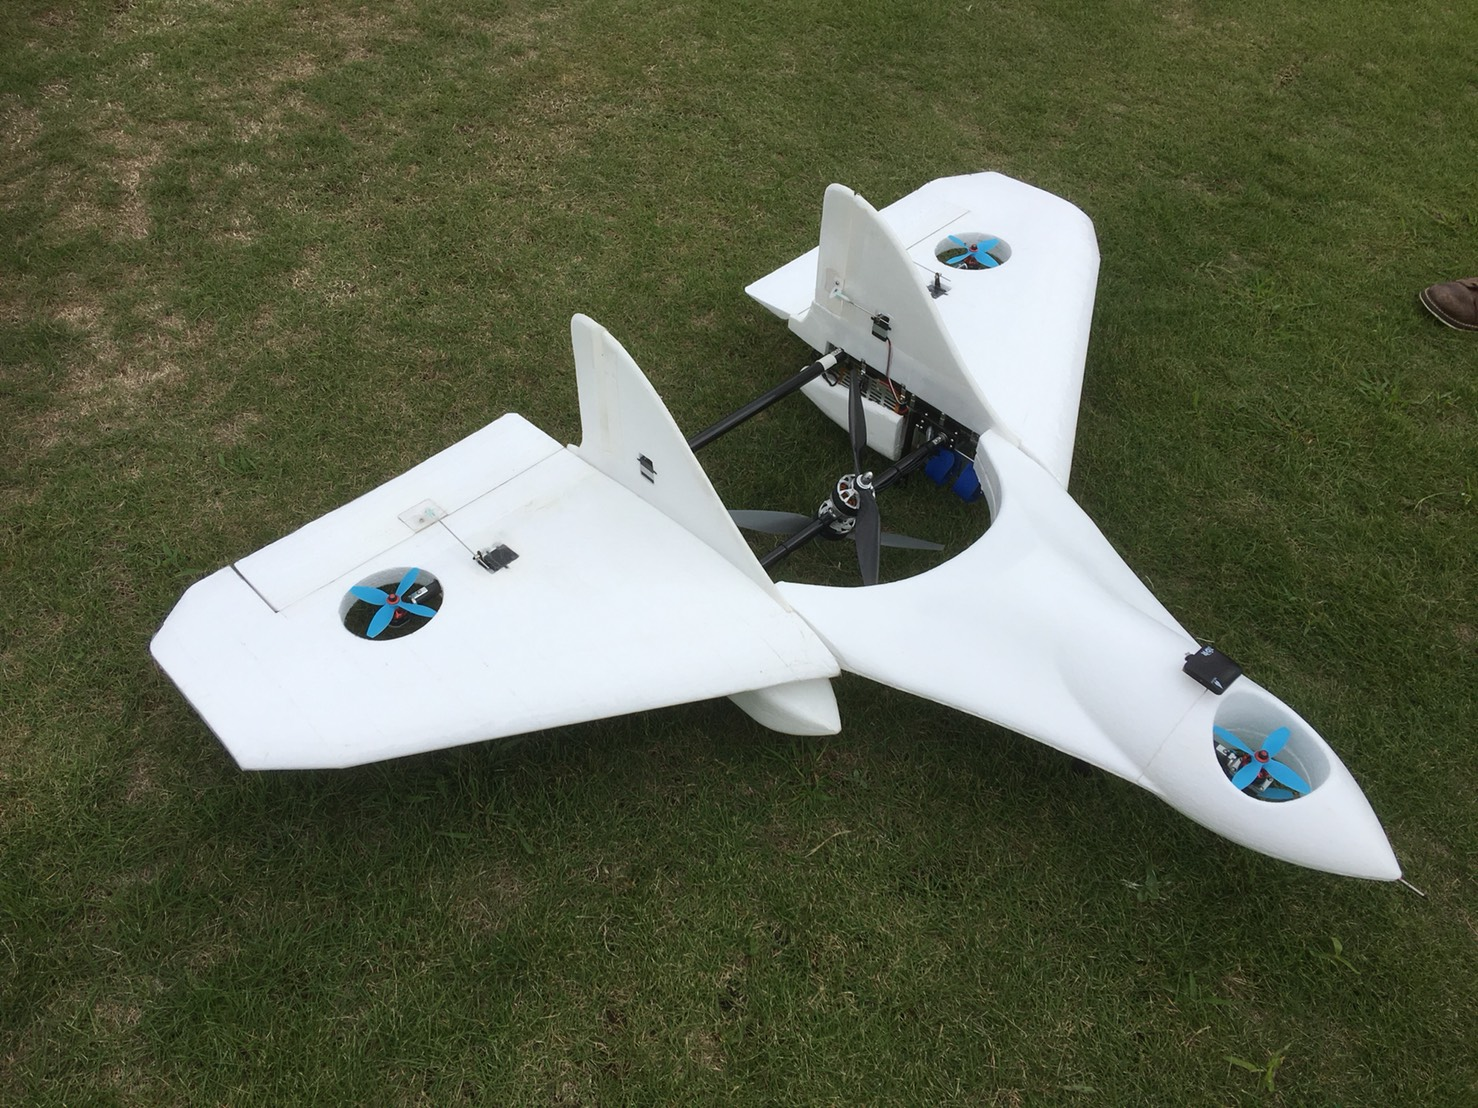
\includegraphics[clip,width=10.0cm]{vtol23K_2.pdf}
\caption{Tilt rotor UAV}
\label{fig:vtol23k}
\end{figure}


\section{搭載システム}
